\documentclass[tikz,border=5mm]{standalone}
\usepackage{xcolor}

\begin{document}
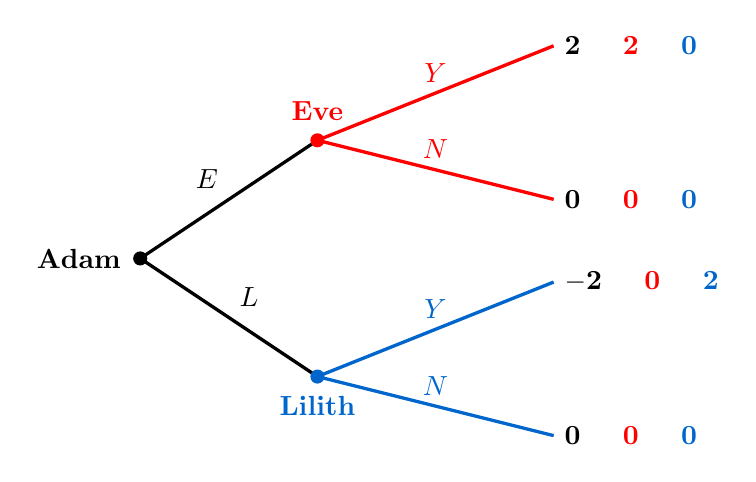
\begin{tikzpicture}[
    scale=1.5,
    font=\bfseries,
    dot/.style={circle, fill=#1, inner sep=1.8pt},
    dot/.default=black,
    line width=1.2pt
]

    % Coordinates
    \coordinate (root)   at (0, 0);
    \coordinate (eve)    at (1.5, 1);
    \coordinate (lilith) at (1.5, -1);
    
    \coordinate (leaf1) at (3.5, 1.8);
    \coordinate (leaf2) at (3.5, 0.5);
    \coordinate (leaf3) at (3.5, -0.2);
    \coordinate (leaf4) at (3.5, -1.5);

    % Level 1 branches (Adam)
    \draw[black] (root) -- (eve)    node[midway, above left] {$E$};
    \draw[black] (root) -- (lilith) node[midway, above right] {$L$};

    % Level 2 branches (Eve - Red)
    \draw[red] (eve) -- (leaf1) node[midway, above] {$Y$};
    \draw[red] (eve) -- (leaf2) node[midway, above] {$N$};

    % Level 2 branches (Lilith - Blue)
    \definecolor{gameblue}{RGB}{0, 102, 204}
    \draw[gameblue] (lilith) -- (leaf3) node[midway, above] {$Y$};
    \draw[gameblue] (lilith) -- (leaf4) node[midway, above] {$N$};

    % Decision Nodes
    \node[dot=black, label=left:Adam] at (root) {};
    \node[dot=red, label={[red]above:Eve}] at (eve) {};
    \node[dot=gameblue, label={[gameblue]below:Lilith}] at (lilith) {};

    % Payoffs (Adam: black, Eve: red, Lilith: blue)
    \node[right] at (leaf1) {2 \quad \textcolor{red}{2} \quad \textcolor{gameblue}{0}};
    \node[right] at (leaf2) {0 \quad \textcolor{red}{0} \quad \textcolor{gameblue}{0}};
    \node[right] at (leaf3) {$-$2 \quad \textcolor{red}{0} \quad \textcolor{gameblue}{2}};
    \node[right] at (leaf4) {0 \quad \textcolor{red}{0} \quad \textcolor{gameblue}{0}};

\end{tikzpicture}
\end{document}
